\documentclass{article}
\title{Numerical Eigenvalue Solver: \\Jacobi's Algorithm Applied to Electrons in a Harmonic Oscillator Potential, and Other Short Stories \smiley\\(Project 2)}
\author{Nat "The Boulder" Hawkins, Victor "From the Streets" Ramirez,\\ Mike "The Pebble" Roosa, Pranjal "Danger" Tiwari}
%the pebble takes issue with this comment

\date{\today}

\usepackage{relsize,makeidx,color,setspace,amsmath,amsfonts,amssymb}
\usepackage[table]{xcolor}
\usepackage{bm,ltablex,microtype}
\usepackage{placeins}
\usepackage{listings}
\usepackage[top = 1in, bottom = 1in, right = 1in, left = 1in]{geometry}
\usepackage[pdftex]{graphicx}
\usepackage{epstopdf}
\usepackage{inputenc}
\usepackage{url}
\usepackage{blindtext}
\usepackage{MnSymbol,wasysym}
\usepackage{MnSymbol,wasysym}
\usepackage[final]{pdfpages}

\begin{document}
\maketitle
\noindent
\begin{abstract}
	The goal of this project is to explore methods of numerical methods and implementing Jacobi's algorithm in Python. We will be investigating the behavior of two electrons in a 3-D harmonic oscillator potential with and without the particles interacting. The physical implications of this relate to the study of quantum dots, which is a popular research topic in physics at the moment. To do this we will be solving the Schr$\ddot{o}$dinger equation. We were able to calculate the eigenvalues for a square symmetric matrix that agree with the eigenvalues of standard python library solvers (i.e. numpy.linalg.eig). We found that with the Jacobi eigensolver, one of the many issues surrounding it is that we do not know the maximum number of iterations needing to be performed on the matrix in question in order to get the eigenvalues. This leads to numerical inefficiencies and illustrates that while this is a valid method, it should not be the primary choice for how to approach this problem. The eigensolver was also used to compute eigenvalues for a specific value of frequency, $\omega$, which we then compared to the analytic results. Our numerical values were within 0.5\% of the analytic value. 
	
\end{abstract}

\newpage

\section{Introduction}

\subsection{Mathematical Motivation}

The aim of this project is to solve Schroedinger's equation for two
electrons in a three-dimensional harmonic oscillator well with and
without a repulsive Coulomb interaction.  We aimed to solve this
equation by reformulating it in a discretized form as an eigenvalue
equation to be solved with Jacobi's method. 

Electrons confined in small areas in semiconductors, so-called quantum
dots, form a hot research area in modern solid-state physics, with
applications spanning from such diverse fields as quantum
nano-medicine to the construction of quantum gates. 

Here we will assume that these electrons move in a three-dimensional harmonic
oscillator potential (they are confined by for example quadrupole fields)
and repel  each other via the static Coulomb interaction.  
We assume spherical symmetry.  

We are first interested in the solution of the radial part of Schr$\ddot{o}$dinger's equation for one electron. This equation reads

\begin{equation*}
  -\frac{\hbar^2}{2 m} \left ( \frac{1}{r^2} \frac{d}{dr} r^2
  \frac{d}{dr} - \frac{l (l + 1)}{r^2} \right )R(r) 
     + V(r) R(r) = E R(r).
\end{equation*}
In our case $V(r)$ is the harmonic oscillator potential $(1/2)kr^2$ with
$k=m\omega^2$ and $E$ is
the energy of the harmonic oscillator in three dimensions.
The oscillator frequency is $\omega$ and the energies are

\begin{equation*}
E_{nl}=  \hbar \omega \left(2n+l+\frac{3}{2}\right),
\end{equation*}
with $n=0,1,2,\dots$ and $l=0,1,2,\dots$.

Since we have made a transformation to spherical coordinates it means that 
$r\in [0,\infty)$.  
The quantum number $l$ is the orbital momentum of the electron.  
% 
Then we substitute $R(r) = (1/r) u(r)$ and obtain
% 

\begin{equation*}
  -\frac{\hbar^2}{2 m} \frac{d^2}{dr^2} u(r) 
       + \left ( V(r) + \frac{l (l + 1)}{r^2}\frac{\hbar^2}{2 m}
                                    \right ) u(r)  = E u(r) .
\end{equation*}
% 
The boundary conditions are $u(0)=0$ and $u(\infty)=0$.

We introduce a dimensionless variable $\rho = (1/\alpha) r$
where $\alpha$ is a constant with dimension length and get
% 

\begin{equation*}
  -\frac{\hbar^2}{2 m \alpha^2} \frac{d^2}{d\rho^2} u(\rho) 
       + \left ( V(\rho) + \frac{l (l + 1)}{\rho^2}
         \frac{\hbar^2}{2 m\alpha^2} \right ) u(\rho)  = E u(\rho) .
\end{equation*}
% 
We will set in this project $l=0$. Inserting $V(\rho) = (1/2) k \alpha^2\rho^2$ we end up with

\begin{equation*}
  -\frac{\hbar^2}{2 m \alpha^2} \frac{d^2}{d\rho^2} u(\rho) 
       + \frac{k}{2} \alpha^2\rho^2u(\rho)  = E u(\rho) .
\end{equation*}
We multiply thereafter with $2m\alpha^2/\hbar^2$ on both sides and obtain

\begin{equation*}
  -\frac{d^2}{d\rho^2} u(\rho) 
       + \frac{mk}{\hbar^2} \alpha^4\rho^2u(\rho)  = \frac{2m\alpha^2}{\hbar^2}E u(\rho) .
\end{equation*}
The constant $\alpha$ can now be fixed so that

\begin{equation*}
\frac{mk}{\hbar^2} \alpha^4 = 1,
\end{equation*}
or

\begin{equation*}
\alpha = \left(\frac{\hbar^2}{mk}\right)^{1/4}.
\end{equation*}
Defining

\begin{equation*}
\lambda = \frac{2m\alpha^2}{\hbar^2}E,
\end{equation*}
we can rewrite Schrodinger's equation as

\begin{equation*}
  -\frac{d^2}{d\rho^2} u(\rho) + \rho^2u(\rho)  = \lambda u(\rho) .
\end{equation*}
This is the first equation to solve numerically. In three dimensions the eigenvalues for $l=0$ are 
$\lambda_0=3,\lambda_1=7,\lambda_2=11,\dots .$

We use the by now standard expression for the second derivative of a function $u$
\begin{equation}
    u''=\frac{u(\rho+h) -2u(\rho) +u(\rho-h)}{h^2} +O(h^2),
    \label{eq:diffoperation}
\end{equation}
where $h$ is our step.
Next we define minimum and maximum values for the variable $\rho$,
$\rho_{\mathrm{min}}=0$  and $\rho_{\mathrm{max}}$, respectively. We needed to check our results for the energies against different values $\rho_{\mathrm{max}}$, since we cannot set $\rho_{\mathrm{max}}=\infty$. For the sake of our initial numerical analysis, we set $\rho_{\mathrm{max}}$=10. In comparing to analytc results at $\omega$=0.25, we set $\rho_{\mathrm{max}}$=40, corresponding to 10 divided by our chosen value of $\omega$. This was as a result of the work done by Taut \cite{journal} and his choice of $\rho_{\mathrm{max}}$, also, we had to choose appropriate values for the interacting case based on our substituions made in order to simplify Schrodinger's Equation for said case.

With a given number of mesh points, $N$, we define the step length $h$ as, with $\rho_{\mathrm{min}}=\rho_0$  and $\rho_{\mathrm{max}}=\rho_N$,

\begin{equation*}
  h=\frac{\rho_N-\rho_0 }{N}.
\end{equation*}
The value of $\rho$ at a point $i$ is then 
\[
    \rho_i= \rho_0 + ih \hspace{1cm} i=1,2,\dots , N.
\]
We can rewrite the Schroedinger equation for a value $\rho_i$ as

\[
-\frac{u(\rho_i+h) -2u(\rho_i) +u(\rho_i-h)}{h^2}+\rho_i^2u(\rho_i)  = \lambda u(\rho_i),
\]
or in  a more compact way

\[
-\frac{u_{i+1} -2u_i +u_{i-1}}{h^2}+\rho_i^2u_i=-\frac{u_{i+1} -2u_i +u_{i-1} }{h^2}+V_iu_i  = \lambda u_i,
\]
where $V_i=\rho_i^2$ is the harmonic oscillator potential.

We define first the diagonal matrix element
\begin{equation*}
   d_i=\frac{2}{h^2}+V_i,
\end{equation*}
and the non-diagonal matrix element
\begin{equation*}
   e_i=-\frac{1}{h^2}.
\end{equation*}
In this case the non-diagonal matrix elements are given by a mere constant.
\emph{All non-diagonal matrix elements are equal}.
With these definitions the Schroedinger equation takes the following form

\begin{equation*}
d_iu_i+e_{i-1}u_{i-1}+e_{i+1}u_{i+1}  = \lambda u_i,
\end{equation*}
where $u_i$ is unknown. We can write the 
latter equation as a matrix eigenvalue problem
\begin{equation}
    \begin{bmatrix}d_0 & e_0 & 0   & 0    & \dots  &0     & 0 \\
                                e_1 & d_1 & e_1 & 0    & \dots  &0     &0 \\
                                0   & e_2 & d_2 & e_2  &0       &\dots & 0\\
                                \dots  & \dots & \dots & \dots  &\dots      &\dots & \dots\\
                                0   & \dots & \dots & \dots  &\dots  e_{N-1}     &d_{N-1} & e_{N-1}\\
                                0   & \dots & \dots & \dots  &\dots       &e_{N} & d_{N}
             \end{bmatrix}  \begin{bmatrix} u_{0} \\
                                                              u_{1} \\
                                                              \dots\\ \dots\\ \dots\\
                                                              u_{N}
             \end{bmatrix}=\lambda \begin{bmatrix} u_{0} \\
                                                              u_{1} \\
                                                              \dots\\ \dots\\ \dots\\
                                                              u_{N}
             \end{bmatrix}.  
      \label{eq:sematrix}
\end{equation}
Since the values of $u$ at the two endpoints are known via the boundary conditions, we can skip the rows and columns that involve these values. Inserting the values for $d_i$ and $e_i$ we have the a matrix form we can now use in Jacobi's Algorithm to solve for the energies. \cite{mortengithub}
The Hamiltonians that we will be concerned with will be in the form of a tridiagonal matrix. We will implement the discretized method to allow for ease of computation via numerical methods.\\
\\
We also studied two electrons in a harmonic oscillator well which also interact via a repulsive Coulomb interaction. We started with the single-electron equation written as
\begin{equation*}
  -\frac{\hbar^2}{2 m} \frac{d^2}{dr^2} u(r) 
       + \frac{1}{2}k r^2u(r)  = E^{(1)} u(r),
\end{equation*}
where $E^{(1)}$ stands for the energy with one electron only. For two electrons with no repulsive Coulomb interaction, we used the following equation
\begin{equation*}
\left(  -\frac{\hbar^2}{2 m} \frac{d^2}{dr_1^2} -\frac{\hbar^2}{2 m} \frac{d^2}{dr_2^2}+ \frac{1}{2}k r_1^2+ \frac{1}{2}k r_2^2\right)u(r_1,r_2)  = E^{(2)} u(r_1,r_2) .
\end{equation*}
Note that we deal with a two-electron wave function $u(r_1,r_2)$ and two electron energy $E^{(2)}$.\\
\\
With no interaction this can be written out as the product of two single-electron wave functions, that is we have a solution on closed form. We introduce the relative coordinate $\mathbf{r} = \mathbf{r}_1-\mathbf{r}_2$
and the center-of-mass coordinate $\mathbf{R} = 1/2(\mathbf{r}_1+\mathbf{r}_2)$. With these new coordinates, the radial Schroedinger equation reads

\begin{equation*}
\left(  -\frac{\hbar^2}{m} \frac{d^2}{dr^2} -\frac{\hbar^2}{4 m} \frac{d^2}{dR^2}+ \frac{1}{4} k r^2+  kR^2\right)u(r,R)  = E^{(2)} u(r,R).
\end{equation*}

The equations for $r$ and $R$ can be separated via the ansatz for the wave function $u(r,R) = \psi(r)\phi(R)$ and the energy is given by the sum of the relative energy $E_r$ and the center-of-mass energy $E_R$, that is
\begin{equation*}
E^{(2)}=E_r+E_R.
\end{equation*}
We add then the repulsive Coulomb interaction between two electrons, namely a term
\begin{equation*}
V(r_1,r_2) = \frac{\beta e^2}{|\mathbf{r}_1-\mathbf{r}_2|}=\frac{\beta e^2}{r},
\end{equation*}
with $\beta e^2=1.44$ eV nm. Adding this term, the $r$-dependent Schroedinger equation becomes

\begin{equation*}
\left(  -\frac{\hbar^2}{m} \frac{d^2}{dr^2}+ \frac{1}{4}k r^2+\frac{\beta e^2}{r}\right)\psi(r)  = E_r \psi(r).
\end{equation*}
This equation is similar to the one we had previously with the noninteracting case and we introduce again a dimensionless variable $\rho = r/\alpha$. Repeating the same steps as we did prior, we arrive at

\begin{equation*}
  -\frac{d^2}{d\rho^2} \psi(\rho) 
       + \frac{1}{4}\frac{mk}{\hbar^2} \alpha^4\rho^2\psi(\rho)+\frac{m\alpha \beta e^2}{\rho\hbar^2}\psi(\rho)  = 
\frac{m\alpha^2}{\hbar^2}E_r \psi(\rho) .
\end{equation*}
We want to manipulate this equation further to make it as similar to the previous equation we solved as possible. We define a new 'frequency'
\begin{equation*}
\omega_r^2=\frac{1}{4}\frac{mk}{\hbar^2} \alpha^4,
\end{equation*}
and fix the constant $\alpha$ by requiring
\begin{equation*}
\frac{m\alpha \beta e^2}{\hbar^2}=1
\end{equation*}
or
\begin{equation*}
\alpha = \frac{\hbar^2}{m\beta e^2}.
\end{equation*}
Defining
\begin{equation*}
\lambda = \frac{m\alpha^2}{\hbar^2}E,
\end{equation*}
we can rewrite Schroedinger's equation as
\begin{equation*}
  -\frac{d^2}{d\rho^2} \psi(\rho) + \omega_r^2\rho^2\psi(\rho) +\frac{1}{\rho} = \lambda \psi(\rho).
\end{equation*}
We treat $\omega_r$ as a parameter which reflects the strength of the oscillator potential.\\
\\
Here we will study the cases $\omega_r=0.25$ for the sake of verifying our results against the analytic results, $\omega_r = 0.01$, $\omega_r = 0.5$, $\omega_r =1$,
and $\omega_r = 5$   
for the ground state only, that is the lowest-lying state.\\
\\
With no repulsive Coulomb interaction we expect to get a result which corresponds to the relative energy of a non-interacting system. \\  
\\
We are only interested in the ground state with $l=0$. We omit the center-of-mass energy. We can reuse the same code, but we need to change the potential from $\rho^2$ to $\omega_r^2\rho^2+1/\rho$. \\
\\
For specific oscillator frequencies, the above equation has answers in an analytical form, see the article by Taut \cite{journal}.\\
\\
The above equations and derivations can be found in the Project 2 assignment sheet on the PHY480 GitHub \cite{mortengithub}.\\
\\
These are the two mathematically distinct cases that we are interested in exploring in our program. Summary of results will be included in our analysis.

\subsection{Methods}
Given this background, we sought to develop a model for the non-interacting and interacting cases of the Schr$\ddot{o}$dinger Equation for two electrons and write an algorithm using the Jacobi Method that would solve for the eigenvalues of a tridiagonal matrix, which is what we expect the Hamiltonian of this system to look like. In the next section, we will discuss how we set up our tridiagonal matrix and how the Jacobi Algorithm solves for the eigenvalues. We ensured that these eigenvalues are accurate by conducting unit tests, such as confirming the orthogonality of our eigenvalues and comparing the eigenvalues that we get from the Jacobi solver with an inbuilt eigensolver in numpy. We also studied the deviation of our calculated results based on varying our parameters as well as the error between our calculated eigenvalues and the accepted values of these eigenvalues according to the literature.\cite{journal}\\
\\
We elected to do this numerical analysis in Python. While we are beginning to become more familiarized with C++, we sought to continue to play to our strengths and produce a Python code for our results. C++ would likely be much more computationally efficient and would allow us to solve larger matrices, but in the interest of advancing our knowledge of Python as well as producing quality results, Python was our choice for programming language.\\
\\
For a good discussion on the Linear Algebra methods explored in this project, a good textbook for reference is G. Strang. \cite{textbook} For a more thorough discussion on the Jacobi Method and other numerical methods that we could have implored for this project, as we will discuss Jacobi's algorithms aren't the most efficient or wisest choice for this type of problem, see Kelley's book on linear and nonlinear methods. \cite{kelley}

\subsection{Development}
In order to achieve the models for non-interacting and interacting electrons, we needed to develop several functions. We found it important to outline the main points about the functions we needed to create prior to the discussion of our work and results. \\
\\
The first function that we needed to define was a function to set up our matrix. This outlines a basic $n$ $\times$ $n$ matrix, which we could outline, that takes in arguments for the potential and outputs a tridiagonal symmetric matrix that we will discuss in our Setup section to come. Then, we set up a function that takes in a tridiagonal matrix and applies the Jacobi algorithm once to provide us with a matrix that is gradually more diagonalized. The calculated eigenvalues converge with each iteration up to a specified decimal point. The final main function we needed to develop was one that would iterate the matrix through the Jacobi algorithm function several times until the largest off diagonal matrix elements fell below our defined value of tolerance ($~10^{-6}-10^{-7}$). The other functions we chose to define performed operations for unit testing, checking for the preservation of orthogonality, and for removing small matrix elements that, after several iterations, became $\approx0$. These will be outlined and commented in our final code and can be seen in the ipython notebook attached at the end of this report. The following sections will discuss the implementation and setup of our algorithms and functions.

\section{Solution}
\subsection{Setup}
We know that the Hamiltonian is a tridiagonal matrix, where the diagonals are 2/$\hbar^2$ +V$_N$ and the elements on either side of the diagonals are -1/$\hbar^2$ for an N$\times$N matrix, is given by multiplying out the matrix from the mathematical motivation (2), is given as:
\[
H=\begin{bmatrix}
\frac{2}{\hbar^2}+V_1 & -\frac{1}{\hbar^2}&0&0&...&0\\
 -\frac{1}{\hbar^2}&\frac{2}{\hbar^2}+V_2& -\frac{1}{\hbar^2}&0&...&0\\
0& -\frac{1}{\hbar^2}&\frac{2}{\hbar^2}+V_3& -\frac{1}{\hbar^2}&...&0\\
0&0&-\frac{1}{\hbar^2}&\frac{2}{\hbar^2}+V_4&...&0\\
...&...&...&...&...&-\frac{1}{\hbar^2}\\
0&0&0&0& -\frac{1}{\hbar^2}&\frac{2}{\hbar^2}+V_{N-1}
\end{bmatrix}
\]
Now we need to find the eigenvalues of this matrix. Throughout the development of our solvers we compared our outputs to that of python's numpy.linalg library functions for unit tests. Specifically, we used it to check the reliability of our Jacobi eigenvalue solver by using it as a reference for eigenvalues. It also provided a convenient means of checking orthogonality throughout the transformations.\\
\\
We began by initializing the matrix for non-interacting electrons in a harmonic oscillator. This simply required adding a  $\frac{1}{\rho^{2}}$ to the potential. One challenge we were faced with in this initialization was the realization of our boundary conditions. We fixed the V[0] and V[n] term to be zero, in accordance to our wave function going to zero at both ends in the limit of Schrodinger's equation and also in accordance with our numerical methods.\\
\\
We then developed the Jacobi algorithm one set of operations at a time on a 2$\times$2 matrix for simplicity. Using the simplified case we developed the functions that located the maximum values and the appropriate trig functions. Since we built our project in a python notebook we had the opportunity to conveniently run unit tests with each new function. For further discussion of unit tests and challenges associated with the development of our code please refer to our python notebooks. \\
\\
When we had finished the Jacobi solver we found that we could produce a diagonal matrix for the 2$\times$2 case in one iteration, but in higher order matrices we would need additional iterations to get the fully diagonalized matrix. As discussed before, we double checked orthogonality for this process and at the end compared our eigenvalues with the linalg output. This was checked for the 2$\times$2 and 3$\times$3 cases before calculating results.\\
\subsection{Jacobi Algorithm}
We chose the Jacobi method to solve for our eigenvalues. The Jacobi method is an iterative method that transforms a symmetric tridiagonal matrix by rotating the matrix until it converges to a solution. G. Strang provides a good discussion of this in his text \cite{textbook}. The algorithm is as follows:

\begin{enumerate}
	\item Search for the largest matrix element $|a_{pq}|$, where indices $p$ and $q$ denote the row and column of the max non-diagonal element of the matrix respectively.
	\item Given $p$ and $q$, we will perform the Jacobi rotation. We define the quantities $s$, $c$, $t$ as $\sin\theta$, $\cos\theta$, and $\tan\theta$ respectively. To obtain s and c, we use the following relationships:
\begin{align*}
	c &= \frac{1}{\sqrt{1+t^{2}}}\\  
	s &= tc 
\end{align*}
    We also define a quantity $\tau$ as:
    
\begin{align*}
	\tau &= \frac{a_{qq} - a_{pp}}{a_{pq}} \ \text{where} \ t^{2} + 2\tau t - 1 = 0. 
\end{align*}
	Truncation errors occur when $\tau$ is very large which skew the value of t and thus s and c. To avoid this, we redefine t as:
	\[
	t = \left\{\begin{array}{lr}
	\frac{1}{\tau+\sqrt{1+\tau^{2}}}, & \text{for } \tau > 0\\
	\frac{1}{-\tau+\sqrt{1+\tau^{2}}}, & \text{for } \tau < 0\\
	\end{array}\right\}
	\]    
    \item We use t and $\tau$ to compute c and s. With values for c and s and indices p and q, we calculate the elements of our new matrix as follows:

\begin{align*}
	b_{ip} &= a_{ip}c - a_{iq}s \ \ \ i \neq p, i \neq q\\
    b_{iq} &= a_{iq}c + a_{ip}s \ \ \ i \neq p, i \neq q \\
    b_{pp} &= a_{pp}c^{2} - 2a_{pq}cs + a_{qq}s^{2}\\ 
    b_{qq} &= a_{pp}s^{2} + 2a_{pq}cs + a_{qq}c^{2}\\
    b_{pq} &= 0\\
    b_{pi} &= b_{ip}\\
    b_{qi} &= b_{iq}
\end{align*}
	The first two expressions transform the tridiagonal elements to converge to 0. The following two expressions are further corrections to the max elements remaining in the matrix. The last expressions "force" the matrix to stay symmetric as the Jacobi method only works for symmetric matrices.
    \item We then repeat 1. and 2. until the largest non-diagonal element $a_{pq}$ is less than some desired accuracy $\epsilon$. We can then read off the eigenvalues as the diagonal elements of the transformed matrix A. 
    

\end{enumerate}
	This method is a straightforward, albeit inefficient way to solve for the eigenvalues. We chose this method for its simplicity as it allowed us to easier understand the nuances of eigenvalue solvers. For future work that requires solving for eigenvalues, it's best to stick to faster algorithms such as the Householder algorithm or use libraries such as numpy's linalg module for Python or armadillo for C++.
    
\subsection{Preservation of Orthogonality and Unit Testing}
A unitary transformation preserves  the orthogonality of the obtained eigenvectors. To see this consider first a basis of vectors $\mathbf{v}_i$,
\[
\mathbf{v}_i = \begin{bmatrix} v_{i1} \\ \dots \\ \dots \\v_{in} \end{bmatrix}
\]
We can assume that the basis is orthogonal, that is 
\[
\mathbf{v}_j^T\mathbf{v}_i = \delta_{ij}.
\]
We set out to show that an orthogonal or unitary transformation
\[
\mathbf{w}_i=\mathbf{U}\mathbf{v}_i,
\]
preserves the dot product and orthogonality.\\
\\
In the code, which will be provided at the end of the report, we implemented multiple unit tests, one of which having to do with the preservation of orthogonality. Out[17] in the Python code below shows the unit test that we performed for a 3$\times$3 matrix we created. This is found on page 8 of 14 in the attached python notebook. The goal was to extract the eigenvectors from the intermediate matrices while we were implementing transformations on the initial 3$\times$3 matrix. The iterative Jacobi solver then returned various dot products every other iteration. If the dot products returned values approximately equal to 0, then the vectors are still orthogonal.\\
\\
The output in Out[17] show that the dot products in our unit test yielded values of the order 10$^{-16}$ or smaller. There is one random output of 0.00372, but this can be explained by a lagging dot product associated with loss of numerical precision at the end of the matrix before the "clean" function is implemented. The clean function merely scans the matrix and removes points set below a certain tolerance, approximately 10$^{-9}$. The values in the matrix were small prior to this cleaning, and the carrying forward floating points, which we found to be a problem in our error analysis in Project 1.\\
\\
We also conducted testing to see whether or not orthogonality was preserved in the matrix that we used to compare to the analytic results. The dot products yield $\approx0$ values. Thus, we could see this preservation of orthogonality in the larger matrices as well as through multiple transformations. See last page of ipython notebook.\\
\\
Multiple other unit tests were performed throughout our analysis. The first 8 input cells of the ipython notebook are actually unit tests of the individual functions before we compiled them into one large function that could fulfill all of the needed tests. We then repeated unit tests of the fully compiled functions for a 2$\times$2 matrix and two 3$\times$3 matrices. This was to test as to whether or not the eigenvalue solver returned the correct eigenvalues without scaling up to the large size matrices. These tests can be seen in outputs, In[8] (page 4 of 14), Out[15] (page 7 of 14), and Out[19] (page 9 of 14). We found that implementing unit tests was critically important for our overall solutions because it allowed for a more step-by-step natured problem-solving environment as well as checking our results before we were no longer able to debug. Unit testing is a useful technique for ensuring proper functionality and will be used for our future projects.\\
\\

\subsection{Comparison to Analytic Solution}
Following the completion of our Jacobi eigenvalue solver, one of the tasks we wanted to complete was to look at how our numerically calculated eigenvalues compared to the analytic solutions provided by Taut \cite{journal}. \\
\\
The example that we chose to evaluate to compare to the analytic solutions was the case where $\omega=0.25$. Taut describes this as $\frac{1}{\omega}$, but in our case it was much simpler to define the value of $\omega$ as we had previously. \\
\\
In this analytic result, the ground state energy, corresponding to the lowest eigenvalue, was given as $\epsilon_{s}=0.6250$. Through our numerical analysis, the Jacobi eigenvalue we created yielded an eigenvalue of 1.2436. There was an ancillary factor of two involved in the way that they defined the rearranged Schr$\ddot{o}$dinger equation. Thus, we yield a final ground state energy, or lowest eigenvalue, of $\epsilon=0.6218$. This gives a $0.5\%$ error when compared to the published analytic result. \\
\\
From this, we can conclude that with proper rescaling of our $\rho_{max}$ value, we can achieve the same results proposed by Taut. With respectably low percent error values as well. In short, our numerical methods are successful in comparison to the published analytic results.

\subsection{Time Comparison}
We evaluated a test for a 40$\times$40 Matrix in the interacting case to see how the Jacobi method compared to the built in eigensolvers that numpy offers. Sample code found in our final program, not the attached pdf ipyhon notebook, yielded the following:
\begin{lstlisting}[language=Python]
A = makemat(40,.25,40)
eigenvals = esolver(A,.00001)
cleaned = clean(eigenvals)
print(cleaned)
[  0.62181583   1.06526775   1.47963271   1.85087367   2.14990337
   2.40874635   2.77068912   3.22976528   3.76667366   4.37568805
   5.05435585   5.80137175   6.61596051   7.49762833   8.44604449
   9.4609788   10.54226605  11.68978461  12.90344296  14.18317098
  15.52891409  16.94062916  18.41828171  19.96184385  21.57129279
  23.24660973  24.98777904  26.79478762  28.66762441  30.60628002
  32.61074643  34.68101672  36.81708493  39.0189459   41.28659509
  43.6200286   46.01925596  48.48604367  51.10945762]
  
  
startJ = time.clock()
esolver(A,.00001)
dTJ = time.clock()-startJ

startL = time.clock()
la.eigvals(A)
dTL = time.clock()-startL

print('Jacobi:',dTJ)
print('Linalg',dTL)

Jacobi: 0.20473100000000066
Linalg 0.0008759999999998769
\end{lstlisting}
The results were surprising to us. We know that our numerical method is not the most computationally efficient method, but we were surprised to see that even for a relatively small matrix, the numpy functions beat Jacobi by 3 orders of magnitude. That means that our numerical approach was approximately 1000$\times$ slower than defined functions already at our disposal. For larger matrices, we expect to run into memory issues when trying to store these matrices.
\\

\subsection{Comparing Results for Different $\omega$}
We wanted to look at some more values aside from $\omega$=0.25, which we used to compare to the analytic results give by Taut. We decided to test $\omega_r = 0.01$, $\omega_r = 0.5$, $\omega_r =1$, and $\omega_r = 5$.

\begin{center}
\begin{tabular}{|c|c|}
\hline
$\omega$&Lowest Eigenvalue, $\epsilon$\\
\hline
0.01&0.10793\\
\hline
0.5&2.2399\\
\hline
1&4.1020\\
\hline
5&17.7836\\
\hline
\end{tabular}
\end{center}

The table above summarizes the results we got for varying values of omega in the interacting case. For low values of $\omega$, we see that the lowest eigenvalues are relatively low, corresponding to low energy systems in the well. As we increase $\omega$ to the order of magnitude of 1, we see eigenvalues similar to the non-interacting case. As omega continues to get larger, the potential well becomes narrower, so our energy values would be expected to be larger because the electrons would be forced to be in close proximity, showing the dominance of the Coulombic repulsion at short distances. Keeping electrons at a short distance would increase their potential energy, so we would expect larger eigenvalues.\\
\\
Now, there could be some issues with our numerical results. Unfortunately, these values of frequency do not correspond to any of the analytic results found by Taut. The values are similar, but his results are for $\omega<$1. This no longer becomes a useful reference for our results when we exceed the maximum $\omega$ values. However, for $\omega$=0.01, which would correspond to 100 in Taut's results, we saw $\epsilon$, the lowest eigenvalue of the system, on the order of Magnitude of 10$^{-2}$, which, if we divide our numerical result in half (as we do in comparing results to Taut based on differences in mathematical assumptions between our approaches), then we see that our lowest eigenvalue is on the same order of magnitude and approximately 0.05, which resembles Taut's results to within 10\%. \cite{journal} This gives us hope in our results that our numerical solutions are approximately correct.\\
\\
Further resources should be sought out to compare the larger values of $\omega$ for comparison sake. We do see the expected trends in our results for varying values of $\omega$. Numerical analysis will be included in the ipython notebook attached to this report.

\section{Future Work}
There are a number of interesting problems that we could look in to exploring more after working on this project. First and foremost, we have a program, albeit an inefficient one, that can solve eigenvalues for a symmetric tridiagonal matrix. This matrix can also be adapted to imbibe any potential we see fit to introduce to the electrons (or other applicable physical scenarios) as well as varying parameters for the given potential, both interacting and non-interacting cases. This could lead to some very interesting results when it comes to electrons in a harmonic oscillator potential. We expect to see the $\frac{1}{r}$ term in the Coulombic potential become dominant and the electrostatic term to dominate in the eigenvalue as we increase the value of $\omega$,corresponding to a wider potential well. Physically speaking, this is where we see the long range coulombic interactions for this force at work. We could conduct some more extensive numerical investigations by scaling our values for $\omega$  in section 2.6 and confirm our hypothesis. \cite{mortengithub} \\
\\
We also only compared a couple of analytic solutions to those provided by Tout. \cite{journal} One in particular for verification that we could get the expected results of $\omega$=0.25. Once we achieved one comparable numerical result, we decided our model could be effectively adapted to coincide with the analytic solutions to this problem. Further work could be conducted for the sake of comparing more results.\\
\\
Further work could be done in translating our program into a C++ program and utilizing this algorithm in conjunction with armadillo (lapack and blas functions) to explore two main ideas. First, how much more efficient is C++ than Python in implementing this algorithm? And, how does the efficiency of the C++ program compare to the armadillo libraries? In Python, we saw that Jacobi's algorithm was not a very efficient means of solving for eigenvalues when compared to the numpy linear algebra functions, and it would be interesting how C++ compares to that

\section{Conclusion}
We have found that the Jacobi method is a slower way of finding the eigenvalues of a matrix compared to the built in eigenvalue solver function. But when we have large matrices, simply storing it could take up a significant amount of memory, which is one of the downfalls of using the built in functions. They require a defined matrix to work, which may be impractical with a sufficiently large matrix. The Jacobi method is one solution to a matrix that is so large that it is not feasible to store it, where we can create a matrix using vectors, while still being able to find eigenvalues to what is returned from the built in functions.\\
\\
We were also able to get comparable results from our model to analytic results and explroe unit testing in our programs. We found unit testing to be invaluable in developing our functions. This will be a concept we carry forward in future numerical work. We offer some ideas for future work and consideration in regards to this problem.\\
\\
All functions and outputs can be referenced in the following ipython notebook and in our source code included in the final project.

\begin{thebibliography}{4}
\bibitem{journal} M. Taut. \textit{Two Electrons in an External Oscillator Potential: Particular Analytic Solutions of a Coulomb Correlation Problem}. Physical Review A, November, 1993.  

\bibitem{mortengithub} Morten Hjorth-Jenson. \textit{PHY 480 Github}.\\ \url{https://github.com/CompPhysics/ComputationalPhysicsMSU}. 2016-2017.

\bibitem{textbook} Strang, G. \textit{Linear Algebra and its Applications, Fourth Edition}. Thomson Learning Inc., 2006.

\bibitem{kelley} Kelley, C.T.. \textit{Iterative Methods for Linear
and Nonlinear Equations}. Society for Industrial and Applied Mathematics, 1995.


\end{thebibliography}

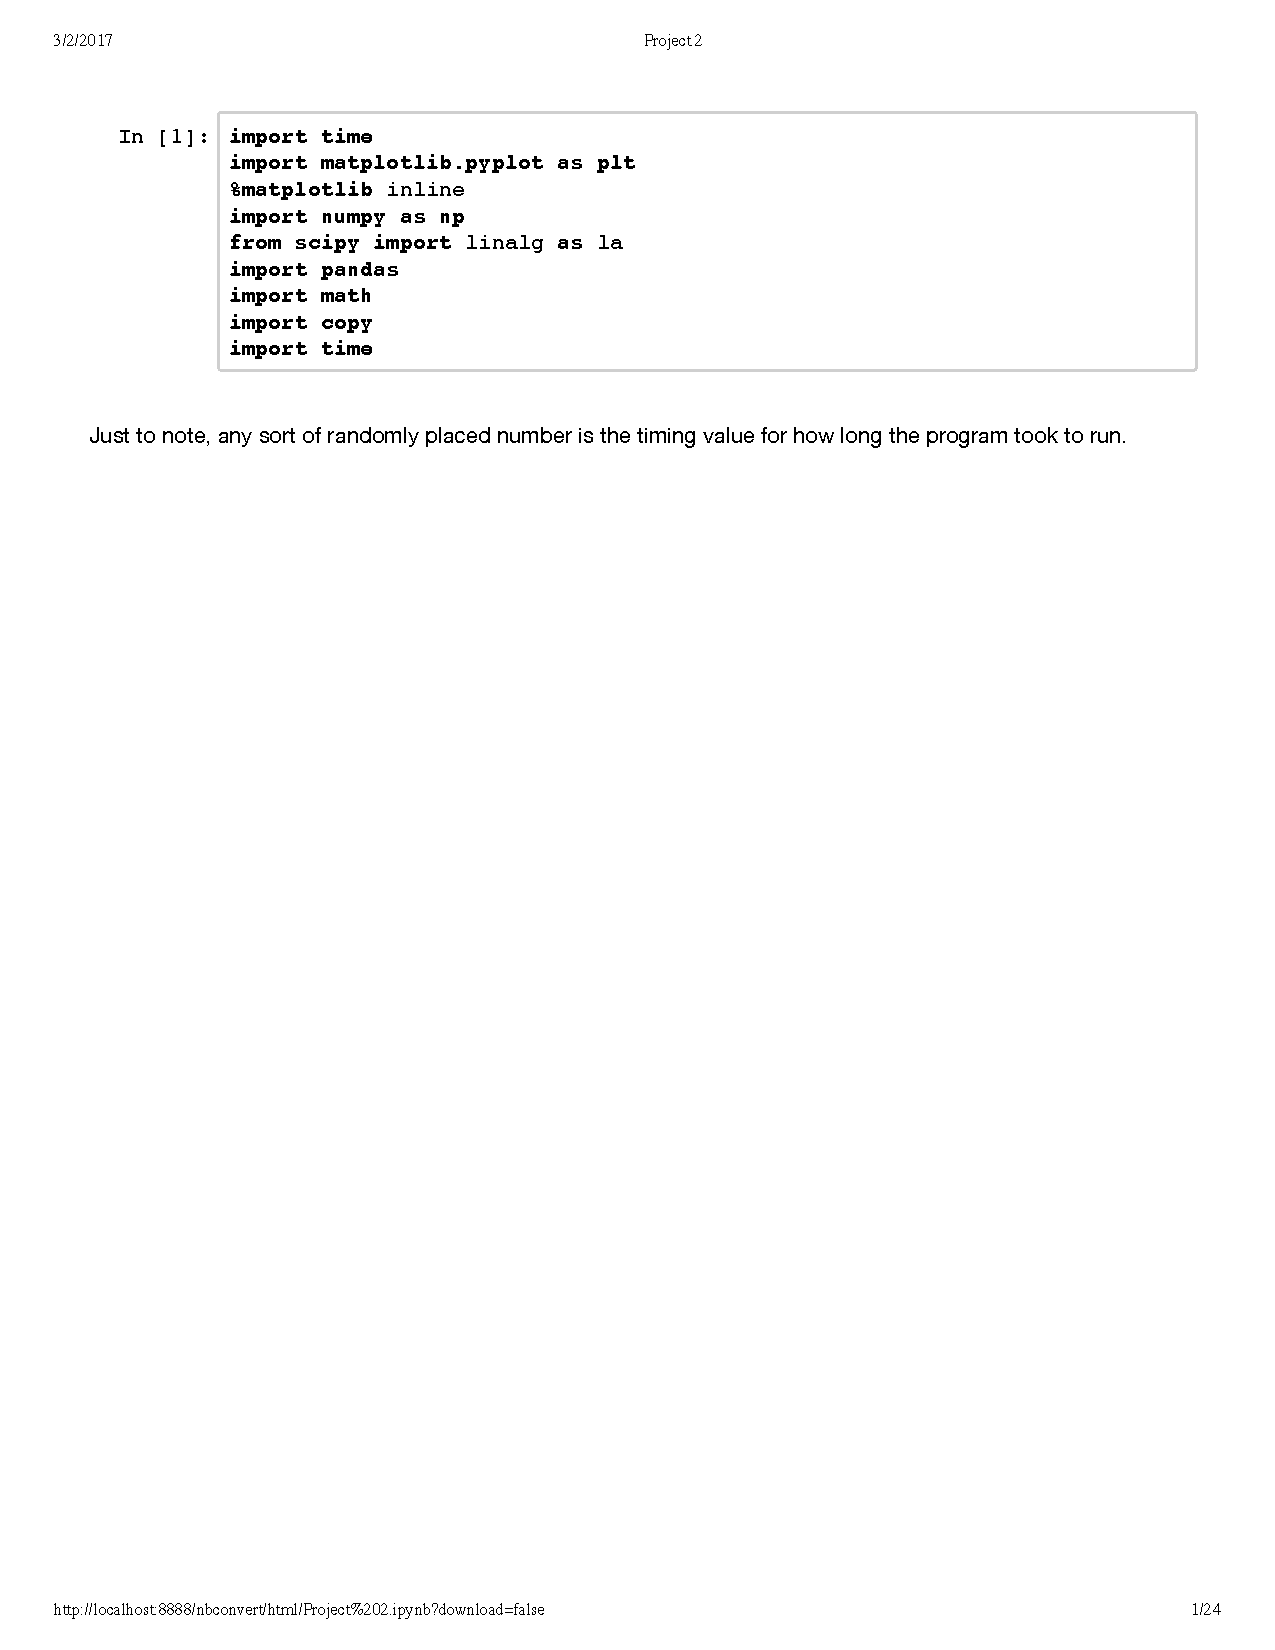
\includepdf[pages=-]{Project2.pdf}

\end{document}